\documentclass{article}
\usepackage{graphicx} % Required for the inclusion of images
\usepackage{natbib} % Required to change bibliography style to APA
\usepackage{amsmath} % Required for some math elements 
\usepackage{wrapfig}
\usepackage{libertine} 
\usepackage{float}
\usepackage{listings}
\usepackage[skip=4pt]{caption}
\usepackage{float}
\usepackage{xcolor}
\usepackage{listings}
\usepackage{xparse}
\usepackage{datetime}

\renewcommand{\today}{\ifcase \month \or January\or February\or March\or %
April\or May \or June\or July\or August\or September\or October\or November\or %
December\fi, \number \year} 
\usepackage[a4paper, margin=1in]{geometry}
\setlength\parindent{0pt} % Removes all indentation from paragraphs

\renewcommand{\labelenumi}{\alph{enumi}.} % Make numbering in the enumerate environment by letter rather than number (e.g. section 6)

%\usepackage{times} % Uncomment to use the Times New Roman font

\title{Neural Networks and Deep Learning \\ Homework 3: Deep Reinforcement Learning}

\author{Giulio \textsc{Zani}} % Author name

\begin{document}

\maketitle

\tableofcontents

\section{Introduction}
OpenAI is a company focused on research in the field of deep learningn. They have devoloped a package called "gym" which offers a fast, computationlly efficient environment to train deep learning agents.
This package has a "step(action)" method which allows one to take an action and observe its conseguence through its output, which consists of:
\begin{itemize}
  \item observation about environmnents
  \item reward 
  \item done (whether it's done playing)
\end{itemize}

In lab 07 professor used a deep Q learning (DQN) algorithm to solve the "Cartpole-v1", a classical problem provided by this package. Here a cart is able to slides frictionlessly and its aim is to keep a pole balanced upward. There are only two possible actions the agent can take, move left or move right. The scope of \textbf{task 1} was to improve the learning procedure given in lab 07.
\begin{figure}[H]
  \begin{center}
    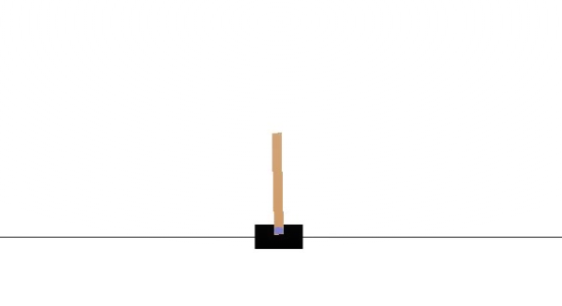
\includegraphics[width=10cm]{imgs/cartpole-v1.png}
    \caption{Rendered frame from Cartpole-v1 problem provided by OpenAI gym package}\label{cartpole-v1}
  \end{center}
\end{figure}
The solution provided by the professor in lab 07 solved the problem by making use of the output of "step(action)" method to get information about the current state. The output is: [cart position, cart velocity, pole angle, pole rotation rate]. The scope of \textbf{task 2} was to instead solve this problem by giving the policy network directly the screen pixels rendered by gym package as an input.
In \textbf{task 3} instead we were allowed to pick another problem provided by the gym package and solve it. I have choosen the "Pendulum-v0" problem.

\section{Task 1: Improving Lab 07 learning procedure}
\subsection{Method}
The first thing that I observed while running the code provided in lab 07 is that the agent was training for a fixed number of episodes, so the training would go on even if the agent was performing maximum score. First thing I have done was to introduce a stopping rule, one that checks the score during a window of episoded and stops training if the agent is scoring (nearly) perfectly. Besides this I changed the optimizer to Adam. 

\subsection{Result}
\begin{figure}[H]
  \begin{center}
    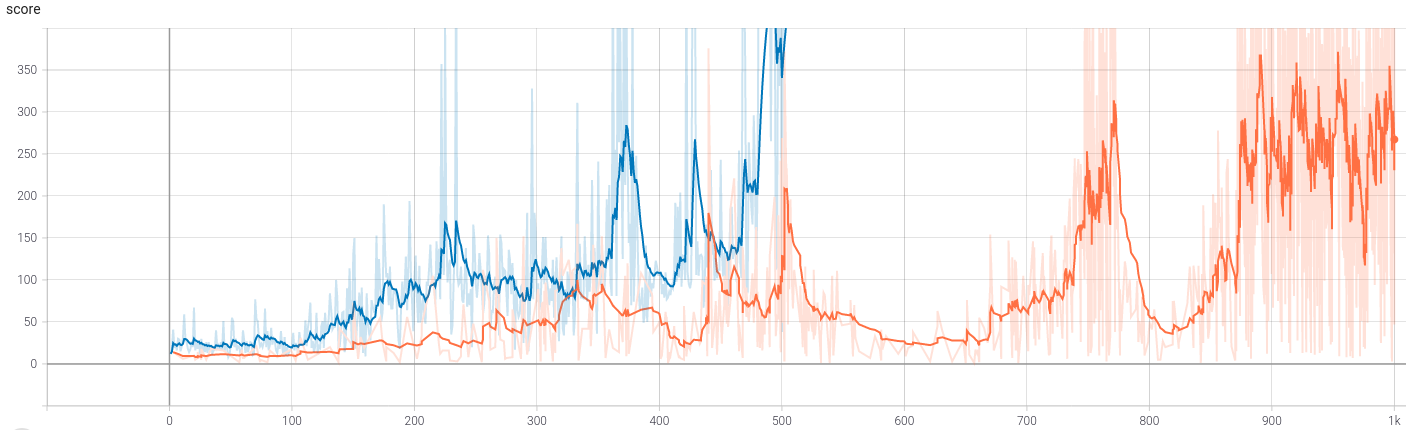
\includegraphics[width=\linewidth]{imgs/task_1_vs_lab_07.png}
    \caption{Score as a function of episode during training in lab 07 (orange) and my improved version for task 1 (blue)}\label{task_1}
  \end{center}
\end{figure}

As one can see in \figurename{\ref{task_1}} Adam optimizer has considerably sped up training and my stopping rule has ended it on time.

\section{Task 2: Solving Cartpole-v1 using screen pixels}
\subsection{Method}
This was for me the most challenging task among the three, mainly due to the long training time needed to solve the problem.

To render the image i have used the method env.render(mode="rgb\_array") of the gym environment. This returns an image in the form of an RGB matrix. Since to solve the problem the agent doesn't need colors I have turned into a greyscale image. I have also shrunk it in size since the original size was way too large and caused the colab gpu to run out of memory. There was however a tradeoff because it's harder detect position with precision from smaller images and larger images slow down the already slow training.

My first naive approach was to just give the current frame as an input to the deep Q policy network. This did not work because the network did not have enough information to solve the problem. The output of the "step(action)" method of the gym package returns not only information about the current cart position, but also information about its first and second derivative. Thus, minim number of frames which the network need to solve the problem are 3. As it turns out however, it's still hard to solve it with 3 so I used 4 to make its life easier.


I have found that convergence to solution for this task was extremely slow (see \figurename{\ref{task_2_training}}), but it seemed that a larger network would converge more reliably (thus the 3 convolutional layers, see the network structure below).
\begin{lstlisting}
Net(
  (conv1): Conv2d(4, 6, kernel_size=(5, 5), stride=(1, 1))
  (pool): MaxPool2d(kernel_size=2, stride=1, padding=0, dilation=1, ceil_mode=False)
  (conv2): Conv2d(6, 16, kernel_size=(5, 5), stride=(1, 1))
  (conv3): Conv2d(16, 20, kernel_size=(5, 5), stride=(1, 1))
  (fc1): Linear(in_features=110500, out_features=2000, bias=True)
  (fc2): Linear(in_features=2000, out_features=500, bias=True)
  (fc3): Linear(in_features=500, out_features=100, bias=True)
  (fc4): Linear(in_features=100, out_features=2, bias=True)
)
\end{lstlisting}

To make sure that the usteady convergence wasn't due to too high LR I have eventually reduced it to 1e-5. While I have reorganised the code I used in task 1 the algorithm logic remains the same, including the stopping rule and Adam optimizer.

\subsection{Result}
\begin{figure}[H]
  \begin{center}
    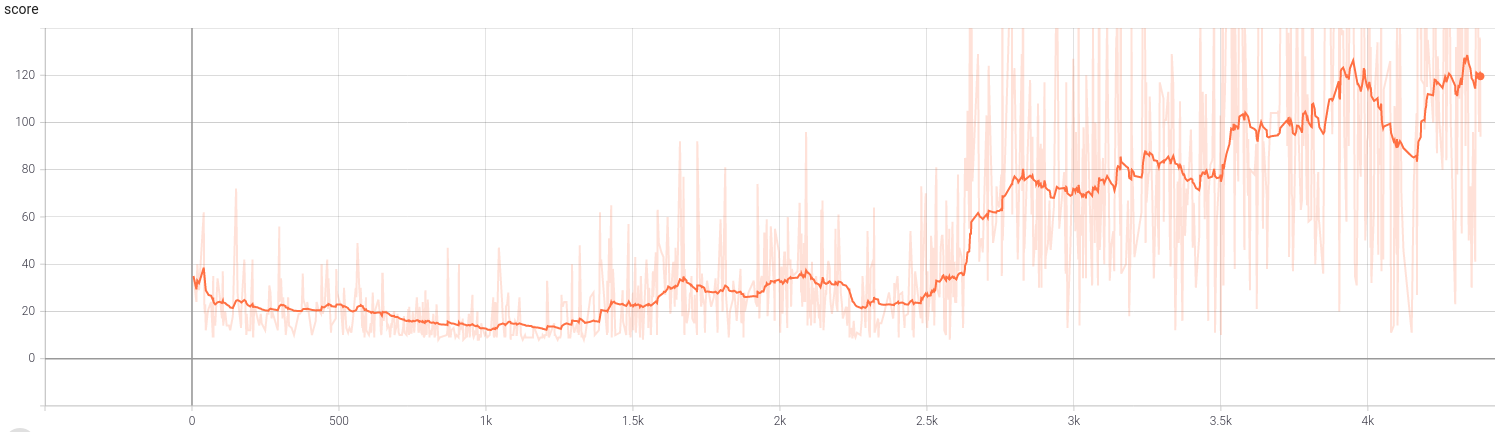
\includegraphics[width=\linewidth]{imgs/task_2_training.png}
    \caption{Partial convergence to the solution in task 2. Notice the short-term decrease in score before the 1.5k episodes. The network probably had to explore quite a bit before finding the solution.}\label{task_2_training}
  \end{center}
\end{figure}
Unfortunately I could not run the training until the end due to time contraints and google colab usage limits. Perhaps fine-tuning further hyperparameters and network structure could speed up training.

\section{Task 3: Solving Pendulum-v0}
\subsection{Introduction}
Pendulum-v0 is another basic reinforcement problem provided by the gym package. 
\begin{figure}[H]
  \begin{center}
    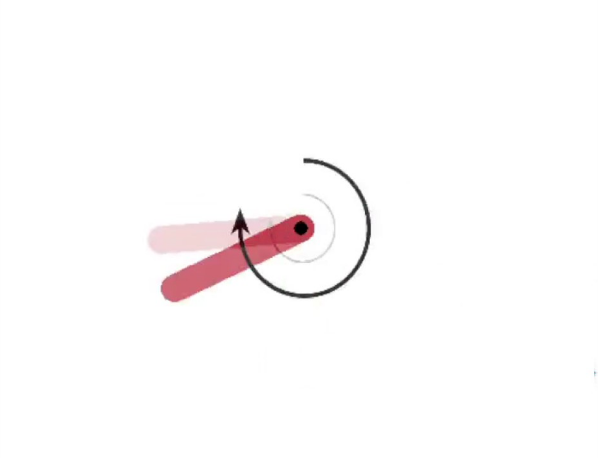
\includegraphics[width=10cm]{imgs/pendulum-v0.png}
    \caption{Pendulum-v0}\label{pendulum_v0}
  \end{center}
\end{figure}
The pendulum starts at a random angle and the agent has to flip it so that the pendulum points upward and keep it in that position for as long as possible. Unlike the Cartpole-v1 here the range of possible actions is a continuum, a force the agent can exert between -2 and +2. The reward is given by the formula:
$$
-(\theta^2 + 0.1*\frac{d \theta}{dt}^2 + 0.001*action^2)
$$
In essence, the goal is to remain at zero angle (vertical), with the least rotational velocity, and the least effort. The maximum possible reward is zero.
\subsection{Method}
To simplify the problem I have sampled the action space, thereby making it descrete with 7 possible actions (evenly spaced within the given range). I have used a very similar algorithm as in Task 1, but I have enlarged the network to make up for the larger action space.

\begin{lstlisting}
DQN(
  (linear): Sequential(
    (0): Linear(in_features=3, out_features=150, bias=True)
    (1): Tanh()
    (2): Linear(in_features=150, out_features=150, bias=True)
    (3): Tanh()
    (4): Linear(in_features=150, out_features=7, bias=True)
  )
)
\end{lstlisting}

\begin{figure}[H]
  \begin{center}
    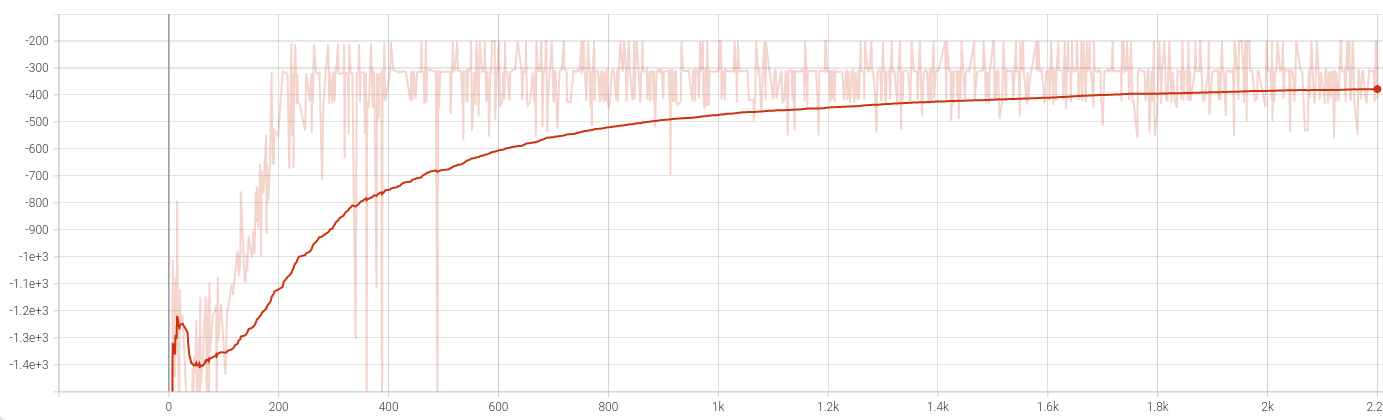
\includegraphics[width=\linewidth]{imgs/task_3_training.png}
      \caption{Score as a function of episode in task 3}\label{task_2_training}
  \end{center}
\end{figure}

For this task I experimented with ReduceLROnPlateau scheduler. I did so because I didn't know which scheduler to use for this particular task and it functioning makes a lot of sense to me. ReduceLROnPlateau automatically reduces the learning rate only if it sees that the loss  I did have to play around with the parameters to get it right though. patience=70 * 200, factor=0.5.

\subsection{Result}
It's hard to get an absolute measure about the results obtained in this task. Unlike the Cartpole-v1 this task doen't have an intrinsic end. So each episode I summed up the rewards and waited until the gym environment reached its maximum number of steps which is 200. I suspect that two things would have been beneficial to improve final results: trying out different network structures and longer training. 

\begin{lstlisting}
EPISODE 1 - FINAL SCORE: -250.5194265625619
EPISODE 2 - FINAL SCORE: -120.90938485976895
EPISODE 3 - FINAL SCORE: -238.50729334666846
EPISODE 4 - FINAL SCORE: -0.7752203254558028
EPISODE 5 - FINAL SCORE: -123.25463520535747
EPISODE 6 - FINAL SCORE: -127.58430355844517
EPISODE 7 - FINAL SCORE: -4.684125804727736
EPISODE 8 - FINAL SCORE: -121.98233763568489
EPISODE 9 - FINAL SCORE: -257.99761994708643
EPISODE 10 - FINAL SCORE: -2.2734690671603
\end{lstlisting}

\end{document}
